\newpage
\begin{center}
  \textbf{\large 1. Техническое задание}
\end{center}
\refstepcounter{chapter}
\addcontentsline{toc}{chapter}{1. ТЕХНИЧЕСКОЕ ЗАДАНИЕ}

Требуется разработать алгоритм для системы позиционирования антенной установки, удовлетворяющий следующим требованиям:

\begin{itemize}[leftmargin=*]
    \item \textbf{Точность наведения}:
    \begin{itemize}[label=--]
        \item Статическая погрешность измерения углового положения: $\leq \pm 1'$ 
        \item Динамическая ошибка сопровождения: $< 1'$ при скорости изменения угла до $30^\circ$/с
    \end{itemize}

    \item \textbf{Алгоритмическое обеспечение}:
    \begin{itemize}[label=--]
        \item Реализация следящего алгоритма
        \item Частота обновления управления: $\geq 10$ кГц
    \end{itemize}
  \end{itemize}
  

  Верификация системы должна быть проведена путем стендовых испытаний с эталонным датчиком.

\noindent\textbf{Критерий успешности}: Система должна обеспечивать непрерывное сопровождение цели с заданной точностью 
в течение всего времени сеанса связи.

\newpage
\begin{center}
  \textbf{\large 2. Общие сведения}
\end{center}
\refstepcounter{chapter}
\addcontentsline{toc}{chapter}{2. ОБЩИЕ СВЕДЕНИЯ}

\section{Организация радиолинии}

Решение задачи организации радиолинии зачастую требует от радиоинженера не только проектирования приемной и передающей антенны, но и учета условий приема. 

В качестве простого примера можно привести абонентскую антенну для приема спутникового телевидения. 
На первый взгляд, задача проста: необходимо разработать зеркальную приемную антенну, диаметр зеркала которой определяется исходя из требования шумовой добротности. 
Вместе с тем, в реальности многие геостационарные спутники, на которые наводится антенна, имеют небольшое наклонение и подвержены возмущениям со стороны Луны и Солнца, 
в связи с чем они описывают на небе фигуры в виде "восьмёрок", вытянутых в направлении север-юг (явление прецессии орбиты). 
В результате прецессии орбиты, точка стояния спутника в картинной плоскости может в течении суток изменяться на 4' – 15', в зависимости от наклонения орбиты. 
Для абонентских антенн, работающих в Ku-диапазоне (12 - 18 ГГц), диаметр зеркала которых равен 0.6м, ширина главного лепестка диаграммы направленности по уровню -3дБ составляет около 150', 
прецессия орбиты геостационарного спутника не оказывает влияние на качество приема сигнала. Следовательно, такая антенна может быть жёстко закреплена к несущей конструкции 
и не требует корректировки своего положения. 

Шлюзовые приемно-передающие антенны, загружающие в геостационарный спутник связи полезный сигнал, чаще всего требуют диаметра зеркала 16м. 
Для такого диаметра зеркала, ширина главного лепестка диаграммы направленности по уровню -3дБ в Ku-диапазоне составляет уже около 6', 
что сопоставимо с величиной движения геостационарного спутника в картинной плоскости в результате прецессии орбиты. 
Более того, применение поляризационного уплотнения требуют высокой величины кросполяризационной развязки (не менее 25дБ). 
Следует отметить, что типовым значением величины кросполяризационной развязки существующих приемо-передающих антенн 
в направлении максимума главного лепестка диаграммы направленности является 27дБ. 

Таким образом, узкая ширина главного лепестка диаграммы направленности, при высоких требованиях к кроссполяризационной развязке, 
приводит к необходимости в оснащении проектируемой антенны опорно-поворотным устройством (ОПУ), оснащённым следящим электроприводом.  
В такой ситуации точность датчиков углового положения электропривода играет важную роль.  

К сожалению, известно весьма немного схем отсчета углового положения осей следящего электропривода. Вместе с тем, для получения сигнала углового положения в тяжелых условиях эксплуатации, 
существует ряд схем, использующих комбинации аналоговых датчиков с аналого-цифровыми преобразователями, одна из которых была реализована.

\section{Анализ типов датчиков углового положения и их применимости в экстремальных условиях}

Современные следящие системы, используемые в зеркальных антенных комплексах, требуют высокой точности и надежности измерений углового положения. 
Для решения этой задачи применяются датчики различных типов, каждый из которых обладает уникальными характеристиками, ограничениями и областью применения. 
Рассмотрим основные категории таких устройств.

\subsection{Oптические энкодеры} 
  
  Эти устройства являются наиболее распространённым решением для измерения угловых перемещений. Принцип действия основан на регистрации светового потока, проходящего через перфорированный диск, 
  закреплённый на валу объекта. Благодаря фотодетекторам, преобразующим световые импульсы в электрические сигналы, можно точно определять положение и скорость вращения.
  Основное достоинство оптических энкодеров заключается в высокой точности (до нескольких угловых секунд) и хорошей разрешающей способности. 
  Однако их работа ограничена условиями эксплуатации: повышенная влажность и температура приводят к образованию конденсата на оптике, 
  что негативно влияет на сигнал и даже может вызвать выход из строя электронного оборудования. 
  Длительное использование в суровых условиях среды ускоряет износ механических элементов и коррозию(рис. ~\ref{Corr}), например, подшипников. В связи с этим возникает необходимость в поддержании нормальных климатических условий,
  что может быть трудновыполнимой задачей в случае, например, дождливых регионов, где приходится применять специальные дегидраторы,(рис. ~\ref{Degidrator1}, \ref{Degidrator2}) 
  или сибирской зимы (см. рис.~\ref{SnowAntenna})

\begin{figure}[htbp]
    \centering
    \begin{minipage}{0.48\linewidth}
       \includegraphics[width=\linewidth]{Сorr1.JPG} 
        
    \end{minipage}\hfill
    \begin{minipage}{0.48\linewidth}
       \centering
        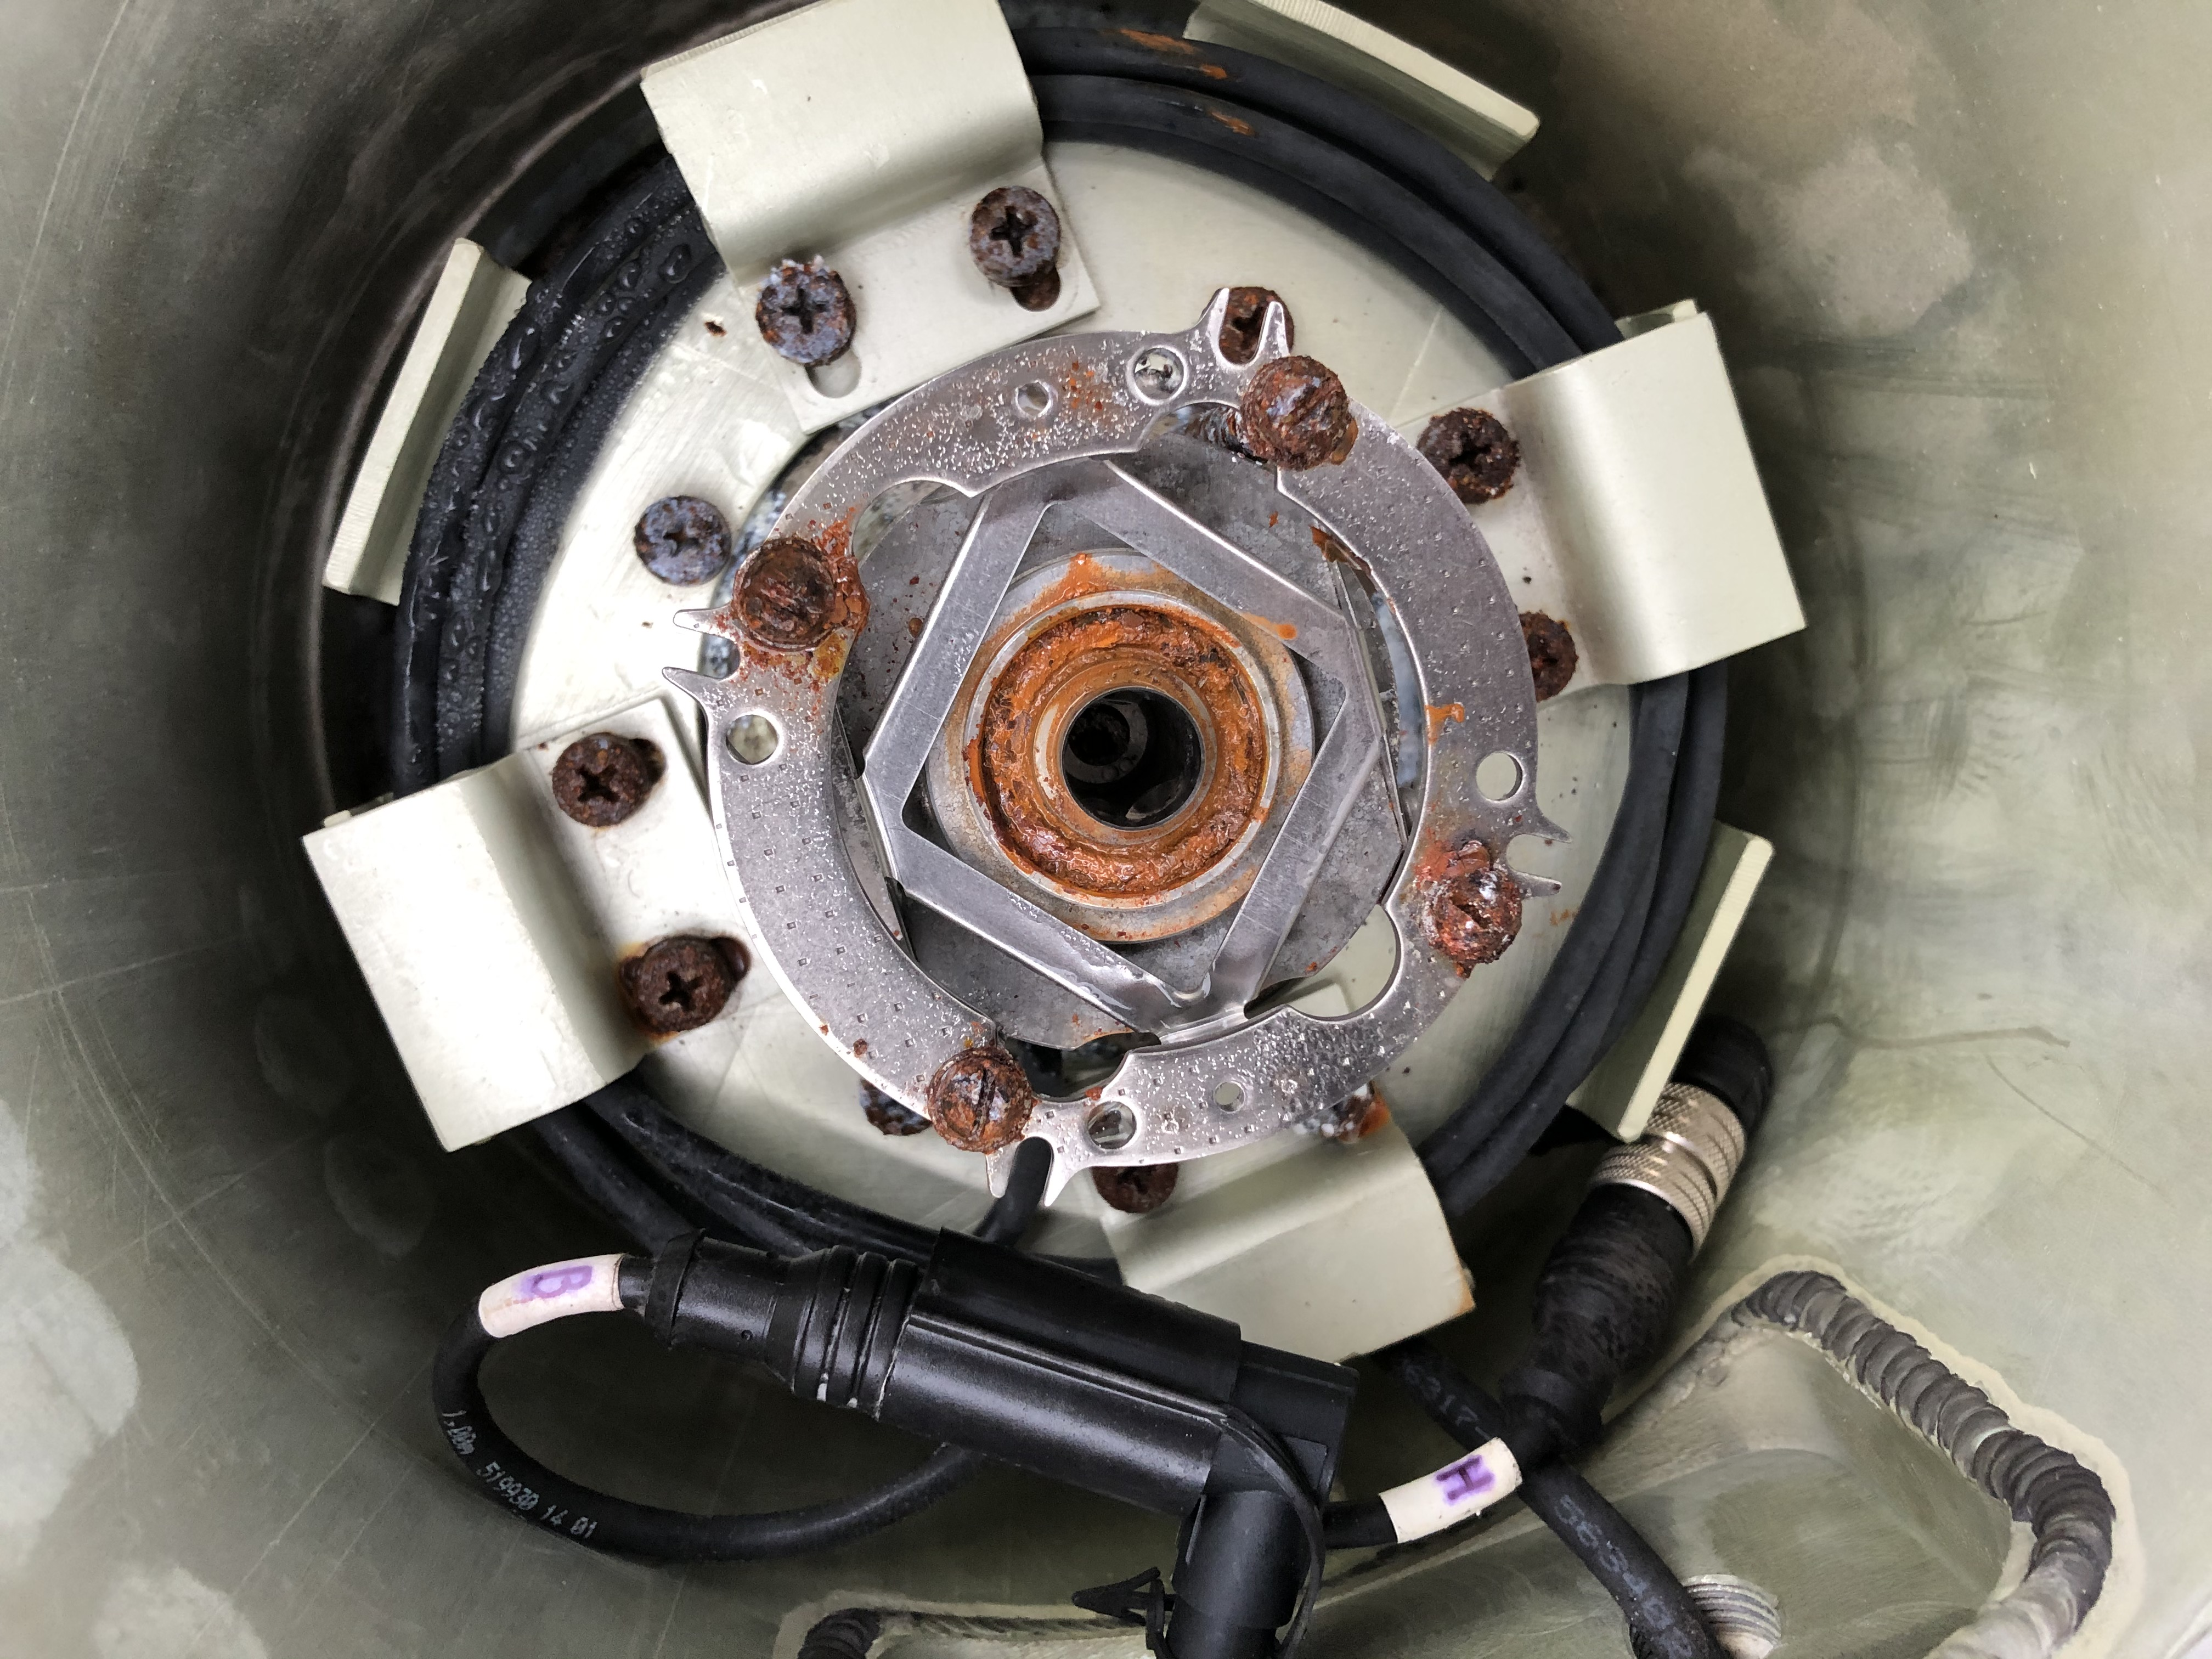
\includegraphics[width=\linewidth]{Corr2.JPG} 
     
    \end{minipage}

    \caption{Коррозия в следствии длительного воздействия агрессивных условий внешней среды}
    \label{Corr}
\end{figure}

\begin{figure}[htbp]
    \centering
    \begin{minipage}{0.48\linewidth}
       \includegraphics[width=\linewidth]{"оптические_энкодеры_в_ОПУ_с_осушением.JPG"} 
        \caption{Оптические энкодеры в ОПУ с осушением}
        \label{Degidrator1} 
    \end{minipage}\hfill
    \begin{minipage}{0.48\linewidth}
       \centering
        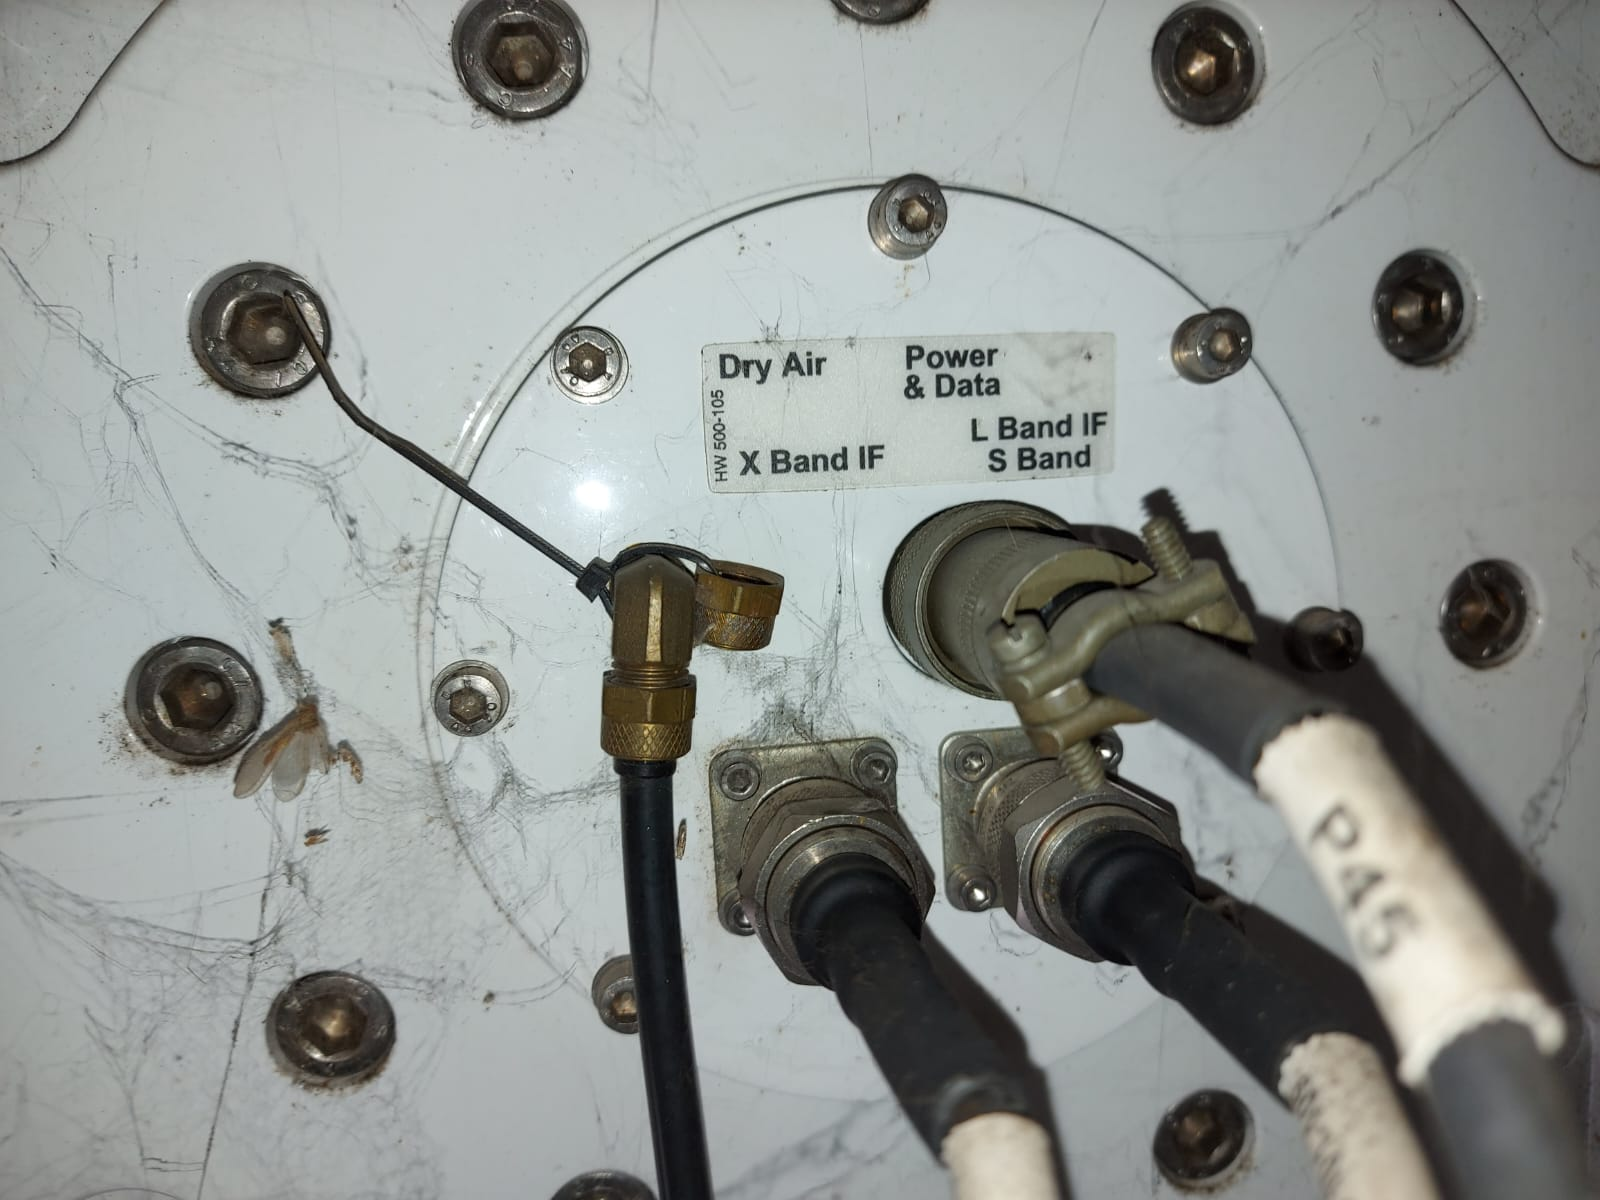
\includegraphics[width=\linewidth]{Подлючение_дегидратора_к_опорно-поворотону_устройству_для_осушения_датчиков.JPG} 
        \caption{Подлючение дегидратора к ОПУ для осушения датчиков}
      \label{Degidrator2}
    \end{minipage}
\end{figure}

\FloatBarrier
 \subsection{Магнитные энкодеры}
  
  Альтернатива оптическим устройствам — магнитные энкодеры, например модель ЛИР-ММ137А, 
  которые используют датчики Холла и магнитные редукторы. Угол поворота измеряется изменением магнитного поля, создаваемого многополюсным магнитом, 
  благодаря чему исключается потребность в оптических компонентах. 
  Это значительно улучшает стойкость к загрязнениям и влагозащиту. 
  Тем не менее, электронные схемы обработки сигналов остаются чувствительными элементами конструкции. 
  Так, низкие температуры вызывают образование льда на проводах и контакты подвергаются коррозии, что ведёт к ошибкам измерений.(рис. \ref{OpuInSnow}) 
  Помимо этого, мощные внешние магнитные поля (например, излучения антенн) оказывают влияние на показания прибора.

  % \begin{figure}[!t]
  %   \centering
  %   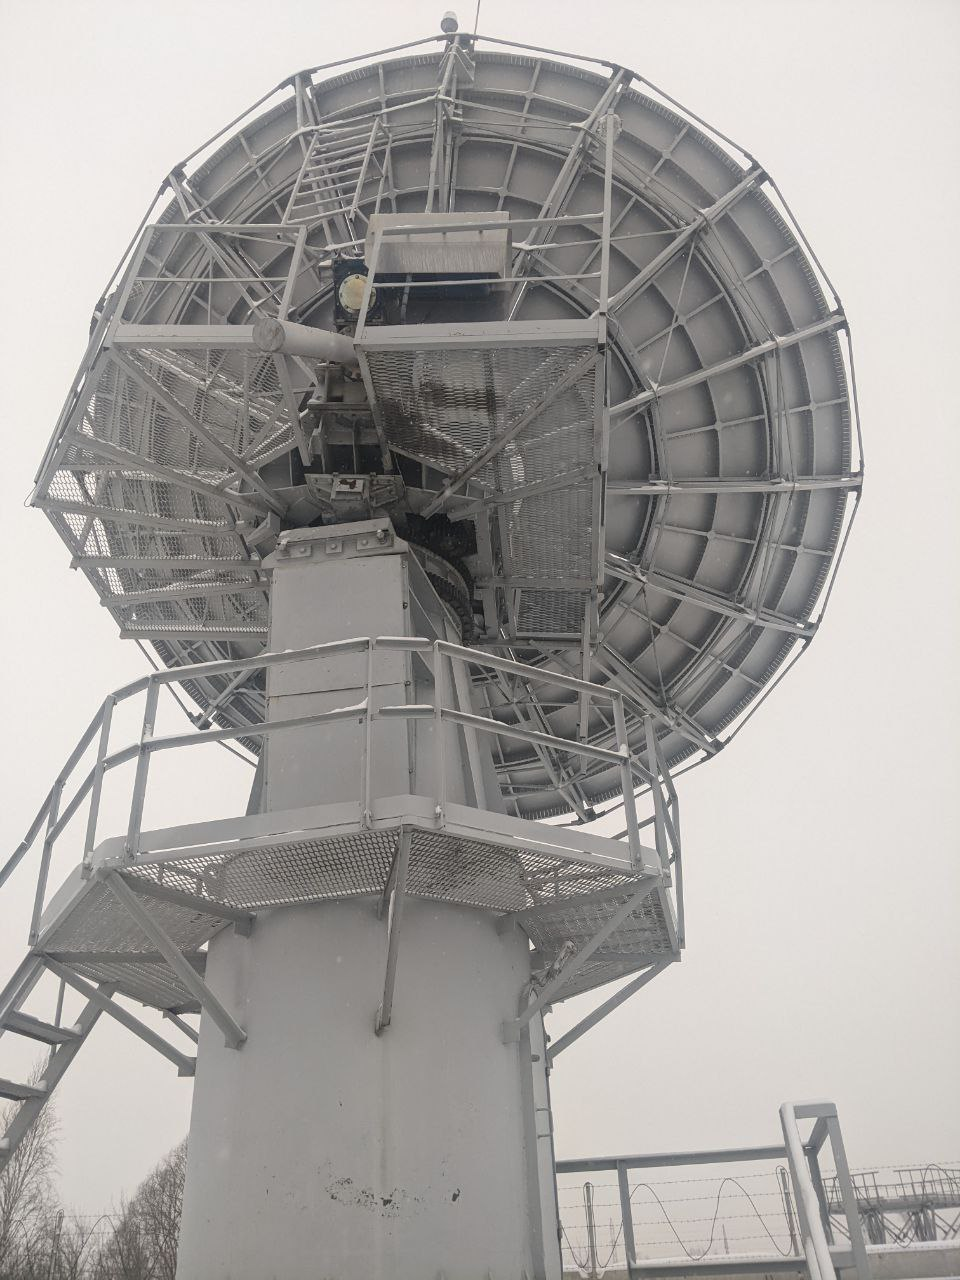
\includegraphics[width=60mm]{SnowAntenna.JPG}
  %   \caption{Антенная система в снегу}
  %   \label{SnowAntenna}
  % \end{figure}

  %  \begin{figure}[!t]
  %   \centering
  %   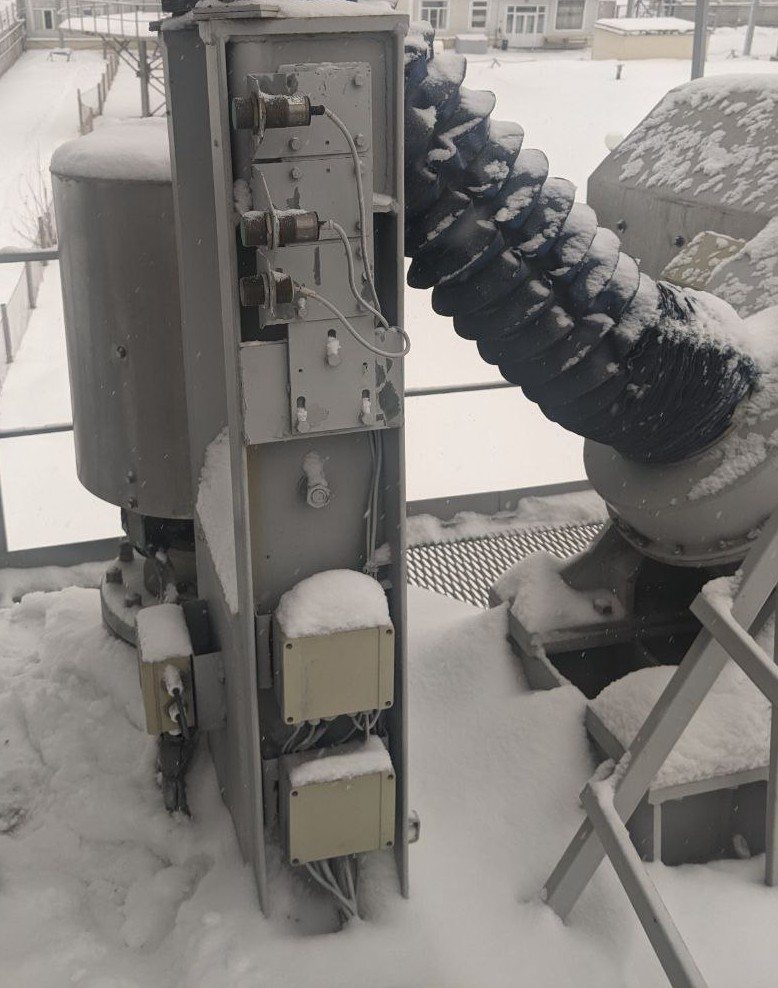
\includegraphics[width=60mm]{OPU.JPG}
  %   \caption{Заснеженные магнитные энкодеры}
  %   \label{OpuInSnow}
  % \end{figure}

  \begin{figure}[htbp]
    \centering
    \begin{minipage}{0.48\linewidth}% ширина первой колонки
        \centering
    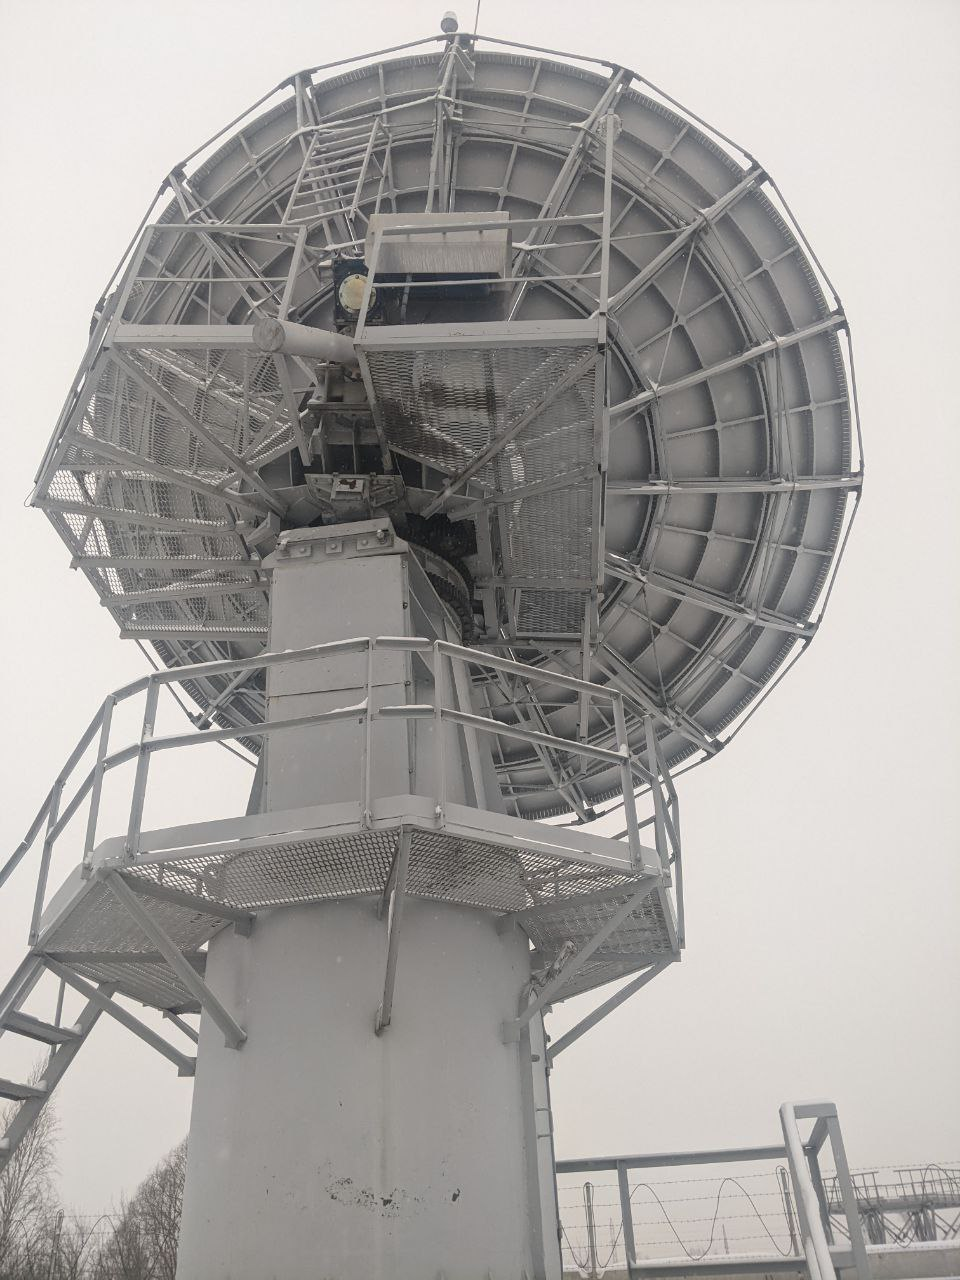
\includegraphics[width=\linewidth]{SnowAntenna.JPG}
    \caption{Антенная система в снегу}
    \label{SnowAntenna}
    \end{minipage}\hfill% добавляем горизонтальное заполнение между изображениями
    \begin{minipage}{0.48\linewidth}% ширина второй колонки
       \centering
    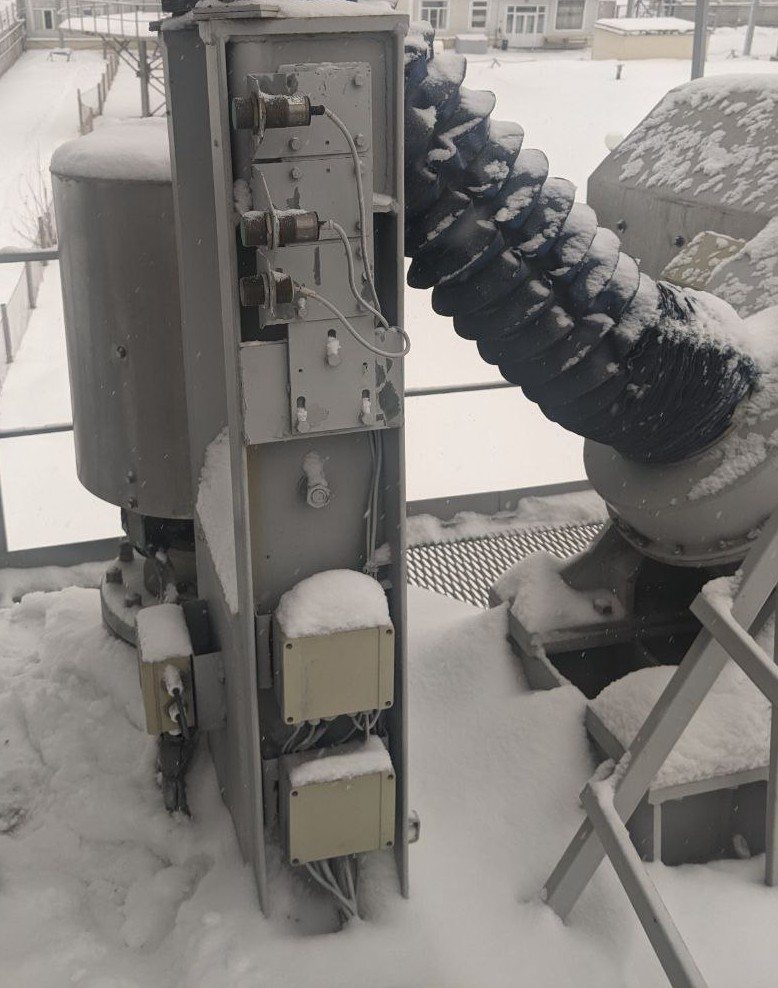
\includegraphics[width=\linewidth]{OPU.JPG}
    \caption{Заснеженные магнитные энкодеры}
    \label{OpuInSnow}
    \end{minipage}
\end{figure}

\FloatBarrier
\subsection{Индукционные датчики углового положения: сельсины, вращающиеся трансформаторы и индуктосины}

Индукционные датчики углового положения, основанные на принципах электромагнитной индукции, являются ключевыми компонентами высоконадежных следящих систем. 
К этой категории относятся: 
\begin{itemize} 
  \item Сельсины 
  \item Вращающиеся трансформаторы (ВТ) 
  \item Индуктосины 
\end{itemize}

Разберем их конструкцию подробнее.

\subsection{Сельсины}

Сельсины — это индукционные машины, преобразующие механический угол поворота в электрический сигнал. Они состоят из пары синхронизированных устройств: датчика (сельсин-датчика) 
и приемника (сельсин-приемника). При изменении угла ротора датчика возникает рассогласование, которое преобразуется в сигнал ошибки, управляющий исполнительным механизмом.
Основное преимущество сельсинов — высокая надежность и устойчивость к вибрациям, влаге и температурным перепадам. Однако их точность ($ \text{не менее}\pm 10 \text{-} 15'$) 
и быстродействие уступают современным требованиям, что ограничивает их применение в высокоточных системах наведения.

\subsection{Вращающиеся трансформаторы (ВТ)}

Вращающиеся трансформаторы — это бесконтактные индукционные датчики, генерирующие сигналы, пропорциональные синусу и косинусу угла поворота вала. 
Благодаря отсутствию электронных компонентов в активной зоне, вращающиеся трансформаторы обладают исключительной устойчивостью к экстремальным условиям: температурам от -60°C до +150°C, 
вибрациям до 100 g и воздействию агрессивных сред.
Точность стандартных моделей вращающихся трансформаторов, таких как ВТ-5 КФ3.031.055, достигает $ \pm 2'$ без дополнительных доработок, 
что удовлетворяет требованиям большинства антенных систем. 
Однако такие устройства, разработанные для военного применения, отличаются высокой стоимостью и длительными сроками поставки (до 12–18 месяцев), 
что делает их малопригодными для гражданских проектов.

Рассмотрим устройство классического вращающегося трансформатора

На cхеме (рис. \ref{SchemeSKVT_Contact}), заимствованной из пособия \cite{AutoDevices} показана конструктивная схема контактного вращающегося трансформатора. 
Магнитопроводы статора 1 и ротора 3 собирают из листов электротехнической стали или пермаллоя, 
изолированных друг от друга лаком. В пазах магнитопроводов статора и ротора размещают по две распределенные обмотки, сдвинутые между собой на 90°. 
Обмотки статора 2 выполняют обычно одинаковыми, т.е. у них совпадает число витков, схема соединения витков и сечение обмоточного провода. 
Одинаковыми изготавливают и роторные обмотки 4. Пространственное расположение обмоток показано на рис. \ref{SchemeSKVT_Contact}; В1 – обмотка возбуждения, В2 – квадратурная обмотка, 
С и К – синусная и косинусная обмотки. Возможны два варианта расположения обмоток: возбуждения и квадратурная (первичные) на статоре, 
синусная и косинусная (вторичные или выходные) на роторе; и наоборот. 

Выводы статорных обмоток подводят непосредственно к соединительным панелям, выводы роторных обмоток вращающихся трансформаторов контактного типа 
выводят через токосъемное устройство: четыре контактных кольца 5 и щетки 6.

В бесконтактных вращающихся трансформаторах напряжения с обмоток ротора можно снимать (подавать) с помощью переходных кольцевых трансформаторов.
В таком вращающемся трансформаторе на месте колец и щеток располагают переходные кольцевые трансформаторы. 
В двухобмоточном кольцевом трансформаторе (рис. \ref{SchemeSKVT}) обмотки 5 и 7 расположены,на кольцевых магнитопроводах 6 и 8 соотвественно.    
Обмотки выполнены в виде сосредоточенных катушек, магнитные оси которых совпадают с направлением вала. Вследствие концентричного расположения при повороте ротора взаимоиндуктивность 
обмоток не меняется. При подаче на статорную обмотку кольцевого трансформатора переменного однофазного напряжения поток $ \Phi_t $ наводит в его роторной обмотке неизменную по амплитуде вторичную ЭДС. 
Соединив проводами роторную обмотку кольцевого трансформатора с одной из основных роторных обмоток вращающегося трансформатора, можно подавать (или снимать) напряжение без колец и щеток. 
Длина бесконтактных вращающихся трансформаторов больше, чем контактных, в связи с необходимостью размещения переходных трансформаторов. Однако существенное повышение надежности 
окупает этот недостаток. Конструкция вращающихся трансформаторов и технология их изготовления должны обеспечивать при повороте ротора изменение взаимоиндуктивности между обмотками статора и ротора по закону, 
наиболее близкому к идеальной синусоиде.



  \begin{figure}[htbp]
    \centering
    \begin{minipage}{0.48\linewidth}% ширина первой колонки
         \centering
          \includegraphics[width=\linewidth]{SchemeSKVT_contact.jpg}
          \caption{Струтурная схема СКВТ}
          \label{SchemeSKVT_Contact}
    \end{minipage}\hfill% добавляем горизонтальное заполнение между изображениями
    \begin{minipage}{0.48\linewidth}% ширина второй колонки
        \centering
        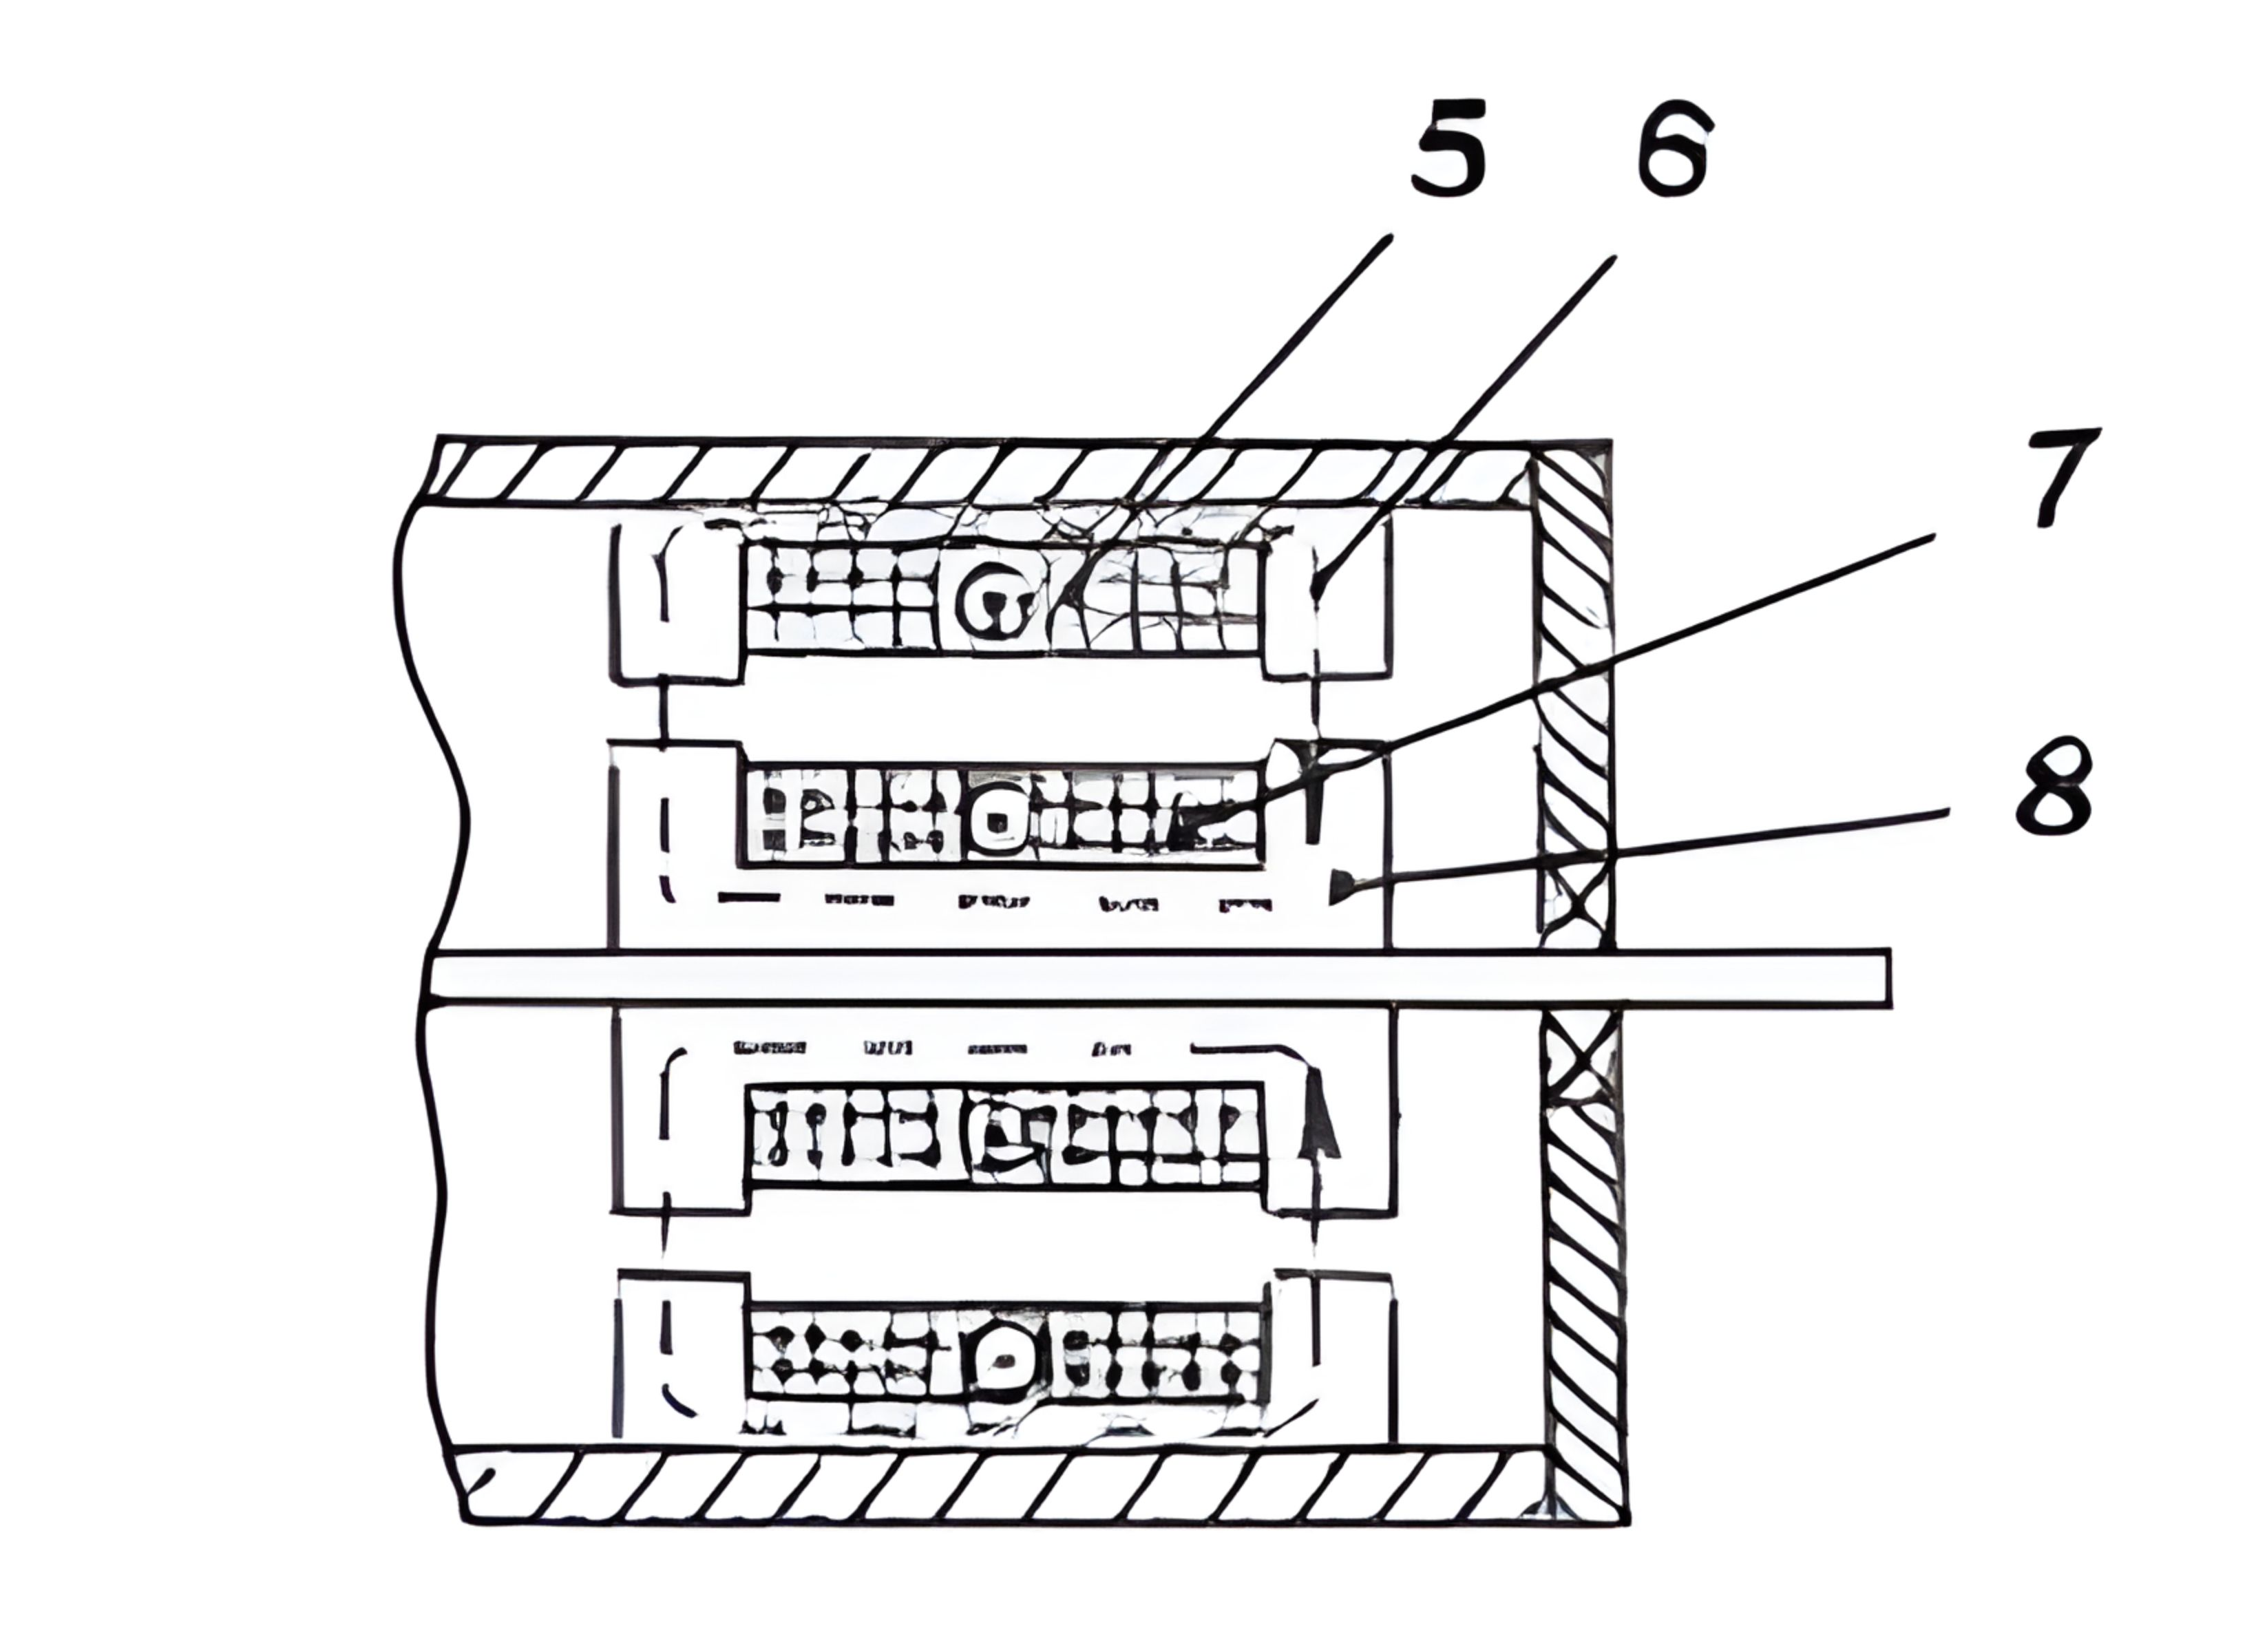
\includegraphics[width=\linewidth]{SchemeSKVT.jpeg}
        \caption{Струтурная схема бесконтактного СКВТ}
        \label{SchemeSKVT}
    \end{minipage}
\end{figure}

\subsubsection{Индуктосины}

Индуктосин — бесконтактный датчик линейного или углового перемещения, работающий на принципе \textbf{модуляции взаимной индуктивности} между обмотками статора 
и подвижной зубчатой частью. 
Основные компоненты индуктосина:
\begin{itemize}
    \item \textbf{Статор} — неподвижная часть с печатными или намотанными обмотками
    \item \textbf{Подвижная часть} (ротор/ползун) — ферромагнитный элемент с зубчатой структурой
    \item \textbf{Ферритовый сердечник} — для концентрации магнитного потока
\end{itemize}


При перемещении зубчатого элемента изменяется магнитное сопротивление цепи. Зоны с зубцом (ферромагнитный материал) и впадиной (воздушный зазор) создают 
периодическую модуляцию потока:

\begin{equation}
    \Phi(x) = \Phi_0 \left[ 1 + m \cdot \sin\left(\frac{2\pi x}{P}\right) \right]
\end{equation}

где:
\begin{itemize}
    \item $\Phi_0$ -- базовый магнитный поток
    \item $m$ -- глубина модуляции (0.2–0.8)
    \item $P$ -- период зубцов
    \item $x$ -- линейное перемещение
\end{itemize}

Основными преимуществами индуктивных датчиков являются бесконтактный принцип работы, исключающий механический износ, и устойчивость к внешним воздействиям — вибрациям, загрязнениям, 
а также возможность эксплуатации в экстремальных условиях (вакуум, агрессивные среды). Благодаря цифровой обработке сигналов система обеспечивает высокую повторяемость измерений 
с точностью до ±0.1 мкм, что критически важно для прецизионных применений в микроэлектронике и робототехнике.

По сравнению с вращающимися трансформаторами индуктивные датчики обладают более высоким разрешением (до 19 бит) и компактными габаритами, что упрощает их интеграцию в миниатюрные устройства. 
Однако  чувствительность к электромагнитным помехам ограничивает использование в промышленных условиях с высоким уровнем шумов, где традиционные вращающиеся трансформаторы 
остаются более надежными.

\section{Проблема выбора доступных решений}
Для гражданских и коммерческих проектов критически важно использование серийно выпускаемых компонентов, которые сочетают надежность, точность и доступность. 
В этом контексте перспективными являются вращающиеся трансформаторы, выпускаемые в стандартизированных корпусах, таких как ROD 426 и ROD 456 от компании Heidenhain. 
Эти габариты соответствуют общепромышленным стандартам, что обеспечивает:

\begin{itemize} 
  \item Совместимость с широким спектром монтажных узлов и редукторов.
  \item Упрощение замены при модернизации систем.
  \item Снижение затрат за счет массового производства и доступности на рынке.
\end{itemize}

Например, ВТ в корпусе ROD 456, несмотря на меньшую точность ($ \pm 5'$), могут быть дополнены двухотсчетной схемой измерения, 
что позволяет повысить разрешающую способность до требуемых значений ($ \pm 2'$).
 \FloatBarrier
\section{Принятое решение по применению датчиков углвого положения}

По результатам проведенного анализа, для повышения надежности электропривода, в качестве измерительных элементов решено использовать общепромышленные и доступные 
синусно-косинусные вращающиеся трансформаторы (резольверы) А12, А13, А27, А29, А40, А42 такие как ЛИР-ДР158А(рис. \ref{LIR} ). Благодаря своей простой конструкции, 
такие датчики углового положения могут без сбоев работать в условиях конденсата. Поскольку погрешность таких датчиков углового положения составляет $ \pm 10'$, 
в целях увеличения точности, измерители углов рассогласования следует выполнять по двухотсчетной схеме с грубым и точным отсчетом и редукцией 1:36. 

  \begin{figure}[!h]
    \centering
    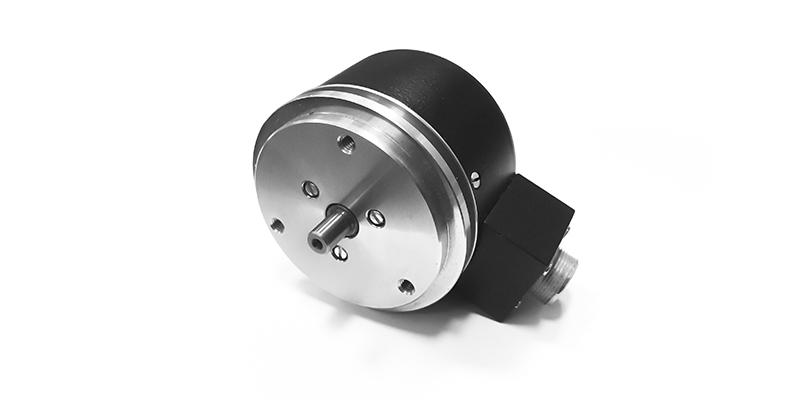
\includegraphics[width=150mm]{ЛИР-ДР158A.jpg}
    \caption{ЛИР-ДР158A}
    \label{LIR}
  \end{figure}

   \FloatBarrier

  